\documentclass[aspectratio=169, 10pt]{beamer}

% ==============================================================================
% IEEE-Style Beamer Presentation for Setquery
% Major Project / B.Tech Defense & Research Symposium
% Assam University, Silchar - Department of Computer Science & Engineering
% ==============================================================================

\usepackage[utf8]{inputenc}
\usepackage[T1]{fontenc}
\usepackage{amsmath, amssymb, amsfonts}
\usepackage{booktabs}
\usepackage{tabularx}
\usepackage{graphicx}
\usepackage{adjustbox}
\usepackage{tikz}
\usetikzlibrary{shapes.geometric, arrows.meta, positioning, calc, fit, backgrounds, shadows}
\usepackage{pgfplots}
\pgfplotsset{compat=1.18}
\usepackage{hyperref}
\usepackage{microtype}
\usepackage{colortbl}
\usepackage{array}

% ------------------------------------------------------------------------------
% Beamer Layout & Margin Settings (Guaranteed Footer Clearance)
% ------------------------------------------------------------------------------
\setbeamersize{text margin left=0.6cm, text margin right=0.6cm}
\addtobeamertemplate{frametitle}{\vspace*{0.05em}}{\vspace*{-0.5em}}

% ------------------------------------------------------------------------------
% IEEE Color Palette & Beamer Theme Settings
% ------------------------------------------------------------------------------
\definecolor{IEEEBlue}{RGB}{0, 102, 153}       % Primary IEEE Cyan-Blue (#006699)
\definecolor{IEEEDarkBlue}{RGB}{0, 40, 85}     % Deep IEEE Navy (#002855)
\definecolor{IEEEAccent}{RGB}{65, 143, 222}    % Soft Highlight Blue
\definecolor{IEEEGray}{RGB}{242, 246, 250}     % Background Card Gray
\definecolor{IEEEDarkGray}{RGB}{70, 80, 95}    % Muted Text Gray
\definecolor{IEEESuccess}{RGB}{34, 139, 34}    % Green (#228B22)
\definecolor{IEEEAlert}{RGB}{178, 34, 34}      % Red Accent (#B22222)
\definecolor{IEEETableHeader}{RGB}{220, 232, 242} % Table Header Background

\setbeamercolor{palette primary}{bg=IEEEDarkBlue, fg=white}
\setbeamercolor{palette secondary}{bg=IEEEBlue, fg=white}
\setbeamercolor{palette tertiary}{bg=IEEEAccent, fg=white}
\setbeamercolor{palette quaternary}{bg=IEEEDarkBlue, fg=white}

\setbeamercolor{structure}{fg=IEEEBlue}
\setbeamercolor{titlelike}{fg=IEEEDarkBlue, bg=white}
\setbeamercolor{frametitle}{fg=white, bg=IEEEDarkBlue}
\setbeamercolor{item}{fg=IEEEBlue}
\setbeamercolor{subitem}{fg=IEEEAccent}

% Block Colors
\setbeamercolor{block title}{bg=IEEEBlue, fg=white}
\setbeamercolor{block body}{bg=IEEEGray, fg=black}
\setbeamercolor{block title alerted}{bg=IEEEAlert, fg=white}
\setbeamercolor{block body alerted}{bg=IEEEGray, fg=black}
\setbeamercolor{block title example}{bg=IEEESuccess, fg=white}
\setbeamercolor{block body example}{bg=IEEEGray, fg=black}

\setbeamertemplate{navigation symbols}{}
\setbeamertemplate{caption}[numbered]

% Clean Header / Footer with Proper Height and Clearance
\setbeamertemplate{headline}{}
\setbeamertemplate{footline}{
  \leavevmode%
  \vspace*{0.2em}%
  \hbox{%
  \begin{beamercolorbox}[wd=.333333\paperwidth,ht=2.2ex,dp=0.8ex,left,leftskip=2ex]{palette primary}%
    \usebeamerfont{author in head/foot}\scriptsize R. Handique, K. Mohanti, T. Purkayastha
  \end{beamercolorbox}%
  \begin{beamercolorbox}[wd=.333333\paperwidth,ht=2.2ex,dp=0.8ex,center]{palette primary}%
    \usebeamerfont{title in head/foot}\scriptsize Setquery --- Assam University
  \end{beamercolorbox}%
  \begin{beamercolorbox}[wd=.333333\paperwidth,ht=2.2ex,dp=0.8ex,right,rightskip=2ex]{palette primary}%
    \usebeamerfont{date in head/foot}\scriptsize 05 Oct 2026\hspace*{2em}
    \insertframenumber{} / \inserttotalframenumber
  \end{beamercolorbox}}%
  \vskip0pt%
}

% ------------------------------------------------------------------------------
% Project Metadata & Author Credentials
% ------------------------------------------------------------------------------
\title[Setquery]{\textbf{Setquery: An Agentic Vision-Language Framework for Multimodal Remote Sensing Intelligence}}
\subtitle{Decoupled Optical, SAR, Bi-Temporal, and Cross-Modal Geophysical Analytics}

\author[Rituraj, Kalyan, Tribikram]{%
  \textbf{Submitted By:}\\[0.2em]
  \textbf{Rituraj Handique} (Roll: 1181200339, Reg: 20230000395)\\[0.1em]
  \textbf{Kalyan Mohanti} (Roll: 1181200340, Reg: 20230000417)\\[0.1em]
  \textbf{Tribikram Purkayastha} (Roll: 11812000324, Reg: 20230000419)
}

\institute[Assam University]{%
  \textbf{Under the Guidance of:} \textbf{Dr. Sunita Sarkar} (Associate Professor)\\[0.2em]
  \textbf{Head of Department:} \textbf{Dr. Tapodhir Acharjee} (Professor \& HOD)\\[0.3em]
  Department of Computer Science and Engineering\\
  Triguna Sen School of Technology\\
  \textbf{Assam University, Silchar --- 788011, India}
}

\date[05 Oct 2026]{Bachelor of Technology in Computer Science \& Engineering $\cdot$ 05 Oct 2026}

% ==============================================================================
\begin{document}

% ------------------------------------------------------------------------------
% Slide 1: Title Slide (Full Institutional Details)
% ------------------------------------------------------------------------------
\begin{frame}[plain]
  \vspace{0.2em}
  \begin{center}
    {\large\textbf{\color{IEEEDarkBlue}ASSAM UNIVERSITY, SILCHAR}}\\[0.15em]
    {\footnotesize\color{IEEEDarkGray}Triguna Sen School of Technology $\cdot$ Department of Computer Science and Engineering}\\[0.25em]
    \hrule height 1.2pt
    \vspace{0.35em}
    {\normalsize\textbf{\color{IEEEBlue}Setquery: An Agentic Vision-Language Assistant for Multimodal Remote-Sensing Imagery Analysis and Evidence-Grounded Query Answering}}\\[0.25em]
    \hrule height 0.8pt
  \end{center}

  \vspace{-0.3em}
  \begin{columns}[T]
    \begin{column}{0.54\textwidth}
      \scriptsize
      \textbf{\color{IEEEDarkBlue}Candidates (B.Tech 2022--2026):}
      \begin{itemize}
        \item \textbf{Rituraj Handique} --- Roll: \texttt{1181200339} (Reg: 20230000395)
        \item \textbf{Kalyan Mohanti} --- Roll: \texttt{1181200340} (Reg: 20230000417)
        \item \textbf{Tribikram Purkayastha} --- Roll: \texttt{11812000324} (Reg: 20230000419)
      \end{itemize}
    \end{column}

    \begin{column}{0.44\textwidth}
      \scriptsize
      \textbf{\color{IEEEDarkBlue}Supervision \& Department:}
      \begin{itemize}
        \item \textbf{Supervisor:} Dr. Sunita Sarkar\\
              \textit{Associate Professor, Dept. of CSE}
        \item \textbf{Head of Dept:} Dr. Tapodhir Acharjee\\
              \textit{Professor \& HOD, Dept. of CSE}
        \item \textbf{Date:} 05 Oct 2026
      \end{itemize}
    \end{column}
  \end{columns}

  \vspace{0.2em}
  \begin{center}
    \tiny\color{IEEEDarkGray}
    \textbf{Focus Areas:} Remote Sensing $\cdot$ Vision-Language Models $\cdot$ Sentinel-1 SAR $\cdot$ Sentinel-2 $\cdot$ ISRO Cartosat/RISAT $\cdot$ Change Detection
  \end{center}
\end{frame}

% ------------------------------------------------------------------------------
% Slide 2: Outline
% ------------------------------------------------------------------------------
\begin{frame}{Presentation Outline}
  \vspace{-0.3em}
  \begin{columns}[T]
    \begin{column}{0.46\textwidth}
      \vspace{0.2em}
      {\small\tableofcontents}
    \end{column}

    \begin{column}{0.52\textwidth}
      \centering
      \adjustbox{max width=\linewidth, max totalheight=0.74\textheight}{%
      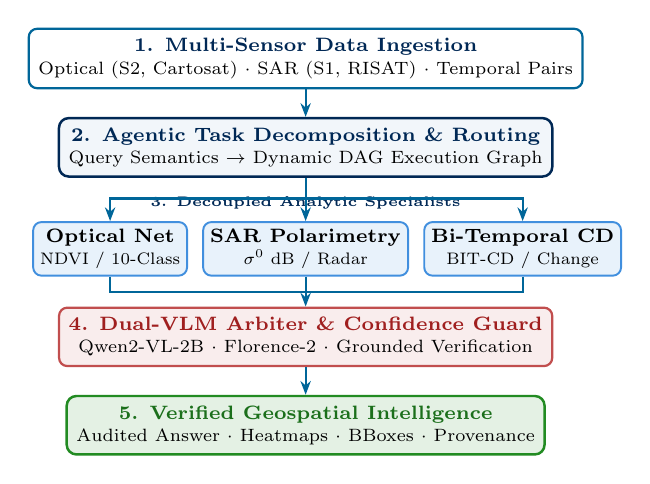
\begin{tikzpicture}[
        font=\scriptsize,
        every node/.style={align=center},
        flowbox/.style={rectangle, draw=IEEEBlue, fill=white, rounded corners=3pt, line width=0.8pt, inner sep=3.5pt, minimum width=5.5cm},
        corebox/.style={rectangle, draw=IEEEDarkBlue, fill=IEEEGray, rounded corners=3.5pt, line width=0.9pt, inner sep=3.5pt, minimum width=5.5cm},
        specbox/.style={rectangle, draw=IEEEAccent, fill=IEEEAccent!12, rounded corners=3pt, line width=0.7pt, inner sep=2.5pt, minimum width=1.7cm, minimum height=0.62cm},
        guardbox/.style={rectangle, draw=IEEEAlert!80, fill=IEEEAlert!8, rounded corners=3pt, line width=0.8pt, inner sep=3.5pt, minimum width=5.5cm},
        outbox/.style={rectangle, draw=IEEESuccess, fill=IEEESuccess!12, rounded corners=3.5pt, line width=0.9pt, inner sep=3.5pt, minimum width=5.5cm},
        arrow/.style={-{Stealth[scale=0.75]}, draw=IEEEBlue, line width=0.8pt}
      ]
        % Node 1: Input & Ingestion
        \node[flowbox] (sensors) {
          \textbf{\color{IEEEDarkBlue}1. Multi-Sensor Data Ingestion}\\
          \scalebox{0.92}{Optical (S2, Cartosat) $\cdot$ SAR (S1, RISAT) $\cdot$ Temporal Pairs}
        };

        % Node 2: Agentic Planning
        \node[corebox, below=0.35cm of sensors] (agent) {
          \textbf{\color{IEEEDarkBlue}2. Agentic Task Decomposition \& Routing}\\
          \scalebox{0.92}{Query Semantics $\to$ Dynamic DAG Execution Graph}
        };

        % Node 3: Specialist Engines (3 sub-blocks side by side)
        \node[specbox, below=0.55cm of agent] (sar) {\textbf{SAR Polarimetry}\\\scalebox{0.86}{$\sigma^0$ dB / Radar}};
        \node[specbox, left=0.18cm of sar] (opt) {\textbf{Optical Net}\\\scalebox{0.86}{NDVI / 10-Class}};
        \node[specbox, right=0.18cm of sar] (cd) {\textbf{Bi-Temporal CD}\\\scalebox{0.86}{BIT-CD / Change}};

        % Label above specialists
        \node[above=0.03cm of sar, font=\tiny\bfseries\color{IEEEDarkBlue}] {3. Decoupled Analytic Specialists};

        % Node 4: Hallucination Guard & Dual-VLM
        \node[guardbox, below=0.38cm of sar] (guard) {
          \textbf{\color{IEEEAlert!90!black}4. Dual-VLM Arbiter \& Confidence Guard}\\
          \scalebox{0.92}{Qwen2-VL-2B $\cdot$ Florence-2 $\cdot$ Grounded Verification}
        };

        % Node 5: Output & Verification
        \node[outbox, below=0.35cm of guard] (output) {
          \textbf{\color{IEEESuccess!80!black}5. Verified Geospatial Intelligence}\\
          \scalebox{0.92}{Audited Answer $\cdot$ Heatmaps $\cdot$ BBoxes $\cdot$ Provenance}
        };

        % Connections
        \draw[arrow] (sensors) -- (agent);

        \coordinate (split) at ($(agent.south)!0.48!(sar.north)$);
        \draw[line width=0.8pt, draw=IEEEBlue] (agent.south) -- (split);
        \draw[arrow] (split) -| (opt.north);
        \draw[arrow] (split) -- (sar.north);
        \draw[arrow] (split) -| (cd.north);

        \coordinate (merge) at ($(sar.south)!0.52!(guard.north)$);
        \draw[line width=0.8pt, draw=IEEEBlue] (opt.south) |- (merge);
        \draw[line width=0.8pt, draw=IEEEBlue] (sar.south) -- (merge);
        \draw[line width=0.8pt, draw=IEEEBlue] (cd.south) |- (merge);
        \draw[arrow] (merge) -- (guard.north);

        \draw[arrow] (guard) -- (output);
      \end{tikzpicture}%
      }
      \vspace{0.15em}\\
      {\tiny\color{IEEEDarkGray}\textbf{Overview:} End-to-end multi-modal remote sensing workflow corresponding to the defense roadmap.}
    \end{column}
  \end{columns}
\end{frame}

% ==============================================================================
\section{Motivation \& Challenges}
% ==============================================================================

\begin{frame}{Motivation: Earth Observation in the Era of VLMs}
  \vspace{-0.2em}
  \begin{columns}[T]
    \begin{column}{0.50\textwidth}
      \textbf{\color{IEEEDarkBlue}Earth Observation (EO) Bottlenecks:}
      \begin{itemize}\setlength{\itemsep}{2.5pt}\small
        \item \textbf{Data Inundation:} Massive daily influx of multispectral (Sentinel-2, Cartosat) and SAR (Sentinel-1, RISAT-1A) satellite rasters.
        \item \textbf{Nadir Perspective Gap:} Standard VLMs (GPT-4V) assume horizontal photography; they fail on top-down scale variance and non-canonical orientations.
        \item \textbf{Multi-Band Incompatibility:} Commercial VLMs accept only 8-bit RGB, failing on 16-bit uint16 GeoTIFFs, NIR/SWIR bands, and radar $\sigma^0_{\text{dB}}$.
        \item \textbf{Hallucination Hazard:} Severe risk of fabricating rivers, runways, or structures in critical defense and flood response.
      \end{itemize}
    \end{column}

    \begin{column}{0.48\textwidth}
      \begin{block}{\small The Setquery Paradigm}
        \begin{itemize}\setlength{\itemsep}{2.5pt}\small
          \item \textbf{Agentic Query Routing:} Decomposes natural language queries into executable multi-specialist DAGs.
          \item \textbf{Decoupled Specialists:} Fine-tuned models dedicated to SAR polarimetry, optical spectral indices, and bi-temporal change.
          \item \textbf{Dual-Engine Fallback:} GPU transformer production backbones paired with deterministic CPU spectral indices (NDVI/Otsu).
          \item \textbf{Auditable Visual Evidence:} Every answer coupled with calibrated confidence, spatial masks, and execution traces.
        \end{itemize}
      \end{block}
    \end{column}
  \end{columns}
\end{frame}

% ==============================================================================
\section{Literature Review \& Gap Analysis}
% ==============================================================================

\begin{frame}{Literature Review: Evolution of Remote Sensing VLMs}
  \vspace{-0.2em}
  \begin{columns}[T]
    \begin{column}{0.50\textwidth}
      \textbf{\color{IEEEDarkBlue}Evolutionary Phases (2020--2024):}
      \begin{itemize}\setlength{\itemsep}{2.5pt}\small
        \item \textbf{RSVQA (Lobry et al., 2020):} Demonstrated that general VQA architectures fail on overhead remote sensing data.
        \item \textbf{RemoteCLIP (Liu et al., 2024):} Contrastive vision-language pretraining for remote sensing (restricted to standard 3-band RGB).
        \item \textbf{GeoChat (CVPR 2024) \& EarthGPT (2024):} Multi-turn instruction-tuned dialogue models; blind to microwave radar physics ($\sigma^0$).
        \item \textbf{BIT-CD (Chen et al., 2022):} Transformer-based bi-temporal change detection over token representations.
      \end{itemize}
    \end{column}

    \begin{column}{0.48\textwidth}
      \begin{alertblock}{\small Core Limitations in Existing Literature}
        \small
        \begin{itemize}\setlength{\itemsep}{2pt}
          \item Treats overhead satellite imagery as standard RGB snapshots, discarding sensor metadata and multi-band radiometry.
          \item Cannot ingest microwave radar backscatter ($\sigma^0$) for cloud-penetrating night/monsoon intelligence.
          \item Confounds seasonal vegetation greening with genuine building structural modifications.
        \end{itemize}
      \end{alertblock}
    \end{column}
  \end{columns}
\end{frame}

% ------------------------------------------------------------------------------
% Slide: Taxonomy & Gap Analysis Table (Guaranteed Zero Footer Collision)
% ------------------------------------------------------------------------------
\begin{frame}{Literature Review: Systematic Taxonomy \& Gap Analysis}
  \vspace{-0.4em}
  \begin{center}
    \adjustbox{max width=0.98\textwidth, max totalheight=0.40\textheight}{%
    \renewcommand{\arraystretch}{1.10}%
    \setlength{\tabcolsep}{4pt}%
    \begin{tabular}{p{4.2cm} c c c c}
      \toprule
      \rowcolor{IEEETableHeader}
      \textbf{Core Architectural Capability} & \textbf{Generic VLMs} & \textbf{RS-VLMs} & \textbf{Specialist Models} & \textbf{Setquery} \\
      \rowcolor{IEEETableHeader}
       & \textit{(GPT-4V, LLaVA)} & \textit{(GeoChat, EarthGPT)} & \textit{(BIT-CD, RemoteCLIP)} & \textbf{(Ours)} \\
      \midrule
      Multispectral Radiometry ($B2\text{--}B8$) & \textcolor{IEEEAlert}{\textbf{No}} & \textcolor{IEEEAlert}{\textbf{No}} & Partial & \textcolor{IEEESuccess}{\textbf{Yes (Sentinel-2 Net)}} \\
      \rowcolor{IEEEGray}
      Calibrated SAR Radar Physics ($\sigma^0$ dB) & \textcolor{IEEEAlert}{\textbf{No}} & \textcolor{IEEEAlert}{\textbf{No}} & \textcolor{IEEEAlert}{\textbf{No}} & \textcolor{IEEESuccess}{\textbf{Yes (Sentinel-1 Net)}} \\
      Optical-SAR Cloud Penetration & \textcolor{IEEEAlert}{\textbf{No}} & \textcolor{IEEEAlert}{\textbf{No}} & \textcolor{IEEEAlert}{\textbf{No}} & \textcolor{IEEESuccess}{\textbf{Yes (AG-MFD Engine)}} \\
      \rowcolor{IEEEGray}
      Phenology vs. Structural Decoupling & \textcolor{IEEEAlert}{\textbf{No}} & Partial & Partial & \textcolor{IEEESuccess}{\textbf{Yes (HSPD Engine)}} \\
      Dual-VLM Mode Collapse Prevention & \textcolor{IEEEAlert}{\textbf{No}} & \textcolor{IEEEAlert}{\textbf{No}} & \textcolor{IEEEAlert}{\textbf{No}} & \textcolor{IEEESuccess}{\textbf{Yes (Qwen2 + Florence)}} \\
      \rowcolor{IEEEGray}
      Open-Vocabulary Visual Grounding & \textcolor{IEEESuccess}{\textbf{Yes}} & Partial & \textcolor{IEEESuccess}{\textbf{Yes}} & \textcolor{IEEESuccess}{\textbf{Yes (Grounding DINO)}} \\
      Auditable Step-by-Step GeoTrace & \textcolor{IEEEAlert}{\textbf{No}} & \textcolor{IEEEAlert}{\textbf{No}} & \textcolor{IEEEAlert}{\textbf{No}} & \textcolor{IEEESuccess}{\textbf{Yes (JSON Trace)}} \\
      \rowcolor{IEEEGray}
      Deterministic CPU Heuristic Fallback & \textcolor{IEEEAlert}{\textbf{No}} & \textcolor{IEEEAlert}{\textbf{No}} & \textcolor{IEEEAlert}{\textbf{No}} & \textcolor{IEEESuccess}{\textbf{Yes (NDVI/Otsu)}} \\
      \bottomrule
    \end{tabular}%
    }
  \end{center}

  \vspace{0.1em}
  \begin{beamercolorbox}[wd=\textwidth, rounded=true, shadow=false, leftskip=2ex, rightskip=2ex]{block body}
    \scriptsize\vspace{0.15em}
    \textbf{\color{IEEEDarkBlue}Core Gaps Resolved:} (1) Full ingestion for multi-band GeoTIFF, Cartosat uint16, and SAR dB $\cdot$ (2) Dynamic agentic dispatch across 6 workflows $\cdot$ (3) Textual claims cross-audited against computed physical indices.\vspace{0.15em}
  \end{beamercolorbox}
\end{frame}

% ==============================================================================
\section{System Architecture \& Workflows}
% ==============================================================================

\begin{frame}{System Architecture: Agentic Multi-Specialist Orchestration}
  \vspace{-0.2em}
  \begin{columns}[T]
    \begin{column}{0.50\textwidth}
      \textbf{\color{IEEEDarkBlue}Core Architectural Tenets:}
      \begin{itemize}\setlength{\itemsep}{2.5pt}\small
        \item \textbf{Decomposition-First:} Ingests unstructured user queries and formulates a structured sub-task DAG.
        \item \textbf{Decoupled Specialists:} Dispatches tasks to domain-dedicated models rather than a single monolithic transformer.
        \item \textbf{Dual-VLM Synthesis:} Blends high-level spatial reasoning (Qwen2-VL-2B) with fine-grained visual grounding (Florence-2).
        \item \textbf{Sensor Normalization:} Dynamic percentile stretching ($P_2$--$P_{98}$) for Cartosat uint16 and decibel conversion for RISAT SAR.
      \end{itemize}
    \end{column}

    \begin{column}{0.48\textwidth}
      \begin{block}{\small Active Specialist Registry}
        \scriptsize
        \begin{itemize}\setlength{\itemsep}{2pt}
          \item \textbf{Single-Image VQA:} RSVQA-adapted transformer.
          \item \textbf{Scene Captioning:} Topographical \& land-cover summarizer.
          \item \textbf{Visual Grounding:} Bounding box $[x_1, y_1, x_2, y_2]$ localization.
          \item \textbf{Bi-Temporal CD:} BIT Siamese transformer \& heatmap.
          \item \textbf{Change VQA:} Temporal delta reasoning.
          \item \textbf{Optical-SAR Fusion:} Cross-modal cloud-penetrating radar.
          \item \textbf{Deterministic Fallback:} NDVI, NDWI, NDBI, Otsu.
        \end{itemize}
      \end{block}
    \end{column}
  \end{columns}
\end{frame}

% ------------------------------------------------------------------------------
% Slide: Agentic Routing Matrix Table (Table 4.1 from Project Report)
% ------------------------------------------------------------------------------
\begin{frame}{Methodology: Agentic Task Routing \& Dispatch Matrix}
  \vspace{-0.4em}
  \begin{center}
    \adjustbox{max width=0.98\textwidth, max totalheight=0.42\textheight}{%
    \renewcommand{\arraystretch}{1.12}%
    \setlength{\tabcolsep}{5pt}%
    \begin{tabular}{p{2.6cm} p{5.6cm} p{4.6cm}}
      \toprule
      \rowcolor{IEEETableHeader}
      \textbf{Input Modality} & \textbf{Query Keyword / Semantic Pattern} & \textbf{Routed Specialist Workflow} \\
      \midrule
      Single Image (Optical) & \textit{``Describe / summarize / land cover / overview''} & Scene Captioning Engine \\
      \rowcolor{IEEEGray}
      Single Image (Optical) & \textit{``Where is / locate / find / bounding box / detect''} & Visual Grounding (Grounding DINO) \\
      Single Image (Optical) & \textit{``What / how many / count / is there / calculate''} & Single-Image VQA (BLIP-2 / Qwen2) \\
      \rowcolor{IEEEGray}
      Bi-Temporal Pair ($T_1, T_2$) & \textit{``What changed / detect modifications / differences''} & Bi-Temporal Change Detection (BIT) \\
      Bi-Temporal Pair ($T_1, T_2$) & \textit{``Why did it change? / was building added?''} & Change VQA (Siamese Reasoning) \\
      \rowcolor{IEEEGray}
      Optical + SAR Pair & \textit{``Fuse SAR / radar penetration / cloud cover''} & Optical-SAR Cross-Modal Fusion \\
      Single / Pair (Any) & \textit{[GPU Unavailable / Low VRAM Condition]} & Deterministic CPU Fallback (NDVI/Otsu) \\
      \bottomrule
    \end{tabular}%
    }
  \end{center}

  \vspace{0.15em}
  \begin{beamercolorbox}[wd=\textwidth, rounded=true, shadow=false, leftskip=2ex, rightskip=2ex]{block body}
    \scriptsize\vspace{0.15em}
    \textbf{\color{IEEEDarkBlue}Autonomous Routing Logic:} The agent extracts intent tokens while verifying CRS alignment across image pairs. If a dedicated GPU is absent, tasks auto-switch to CPU spectral indices without error.\vspace{0.15em}
  \end{beamercolorbox}
\end{frame}

% ------------------------------------------------------------------------------
% Flowchart 1: End-to-End Pipeline
% ------------------------------------------------------------------------------
\begin{frame}{Flowchart 1: End-to-End Agentic Execution Pipeline}
  \centering
  \adjustbox{max width=0.96\textwidth, max totalheight=0.50\textheight}{%
  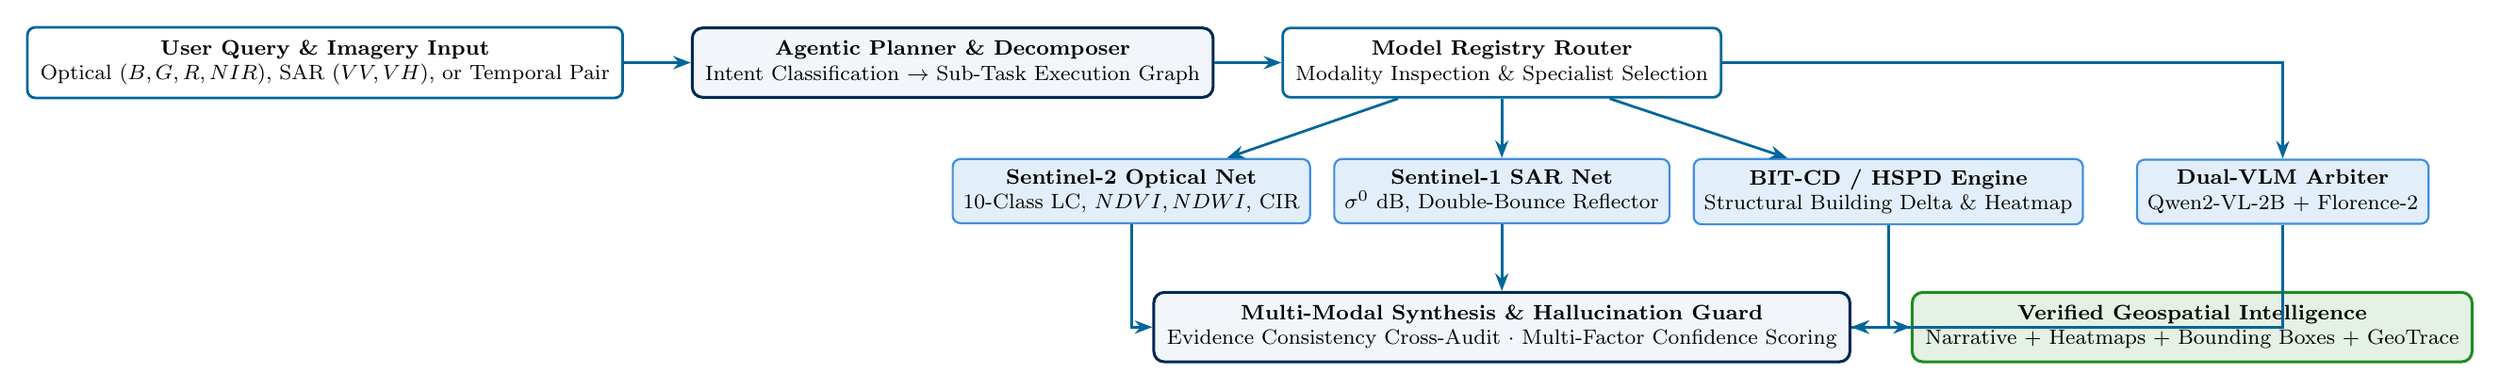
\begin{tikzpicture}[
    node distance=0.6cm and 0.8cm,
    every node/.style={font=\footnotesize, align=center},
    inputbox/.style={rectangle, draw=IEEEBlue, fill=white, rounded corners=3pt, line width=1pt, inner sep=5pt, minimum height=0.85cm},
    agentbox/.style={rectangle, draw=IEEEDarkBlue, fill=IEEEGray, rounded corners=4pt, line width=1.1pt, inner sep=5pt, minimum height=0.85cm},
    specbox/.style={rectangle, draw=IEEEAccent, fill=IEEEAccent!15, rounded corners=3pt, line width=0.8pt, inner sep=4pt, minimum height=0.8cm},
    outbox/.style={rectangle, draw=IEEESuccess, fill=IEEESuccess!12, rounded corners=4pt, line width=1.1pt, inner sep=5pt, minimum height=0.85cm},
    arrow/.style={-{Stealth[scale=0.9]}, draw=IEEEBlue, line width=1pt}
  ]
    % Row 1: Ingestion & Routing
    \node[inputbox] (input) {\textbf{User Query \& Imagery Input}\\Optical ($B,G,R,NIR$), SAR ($VV,VH$), or Temporal Pair};
    \node[agentbox, right=0.9cm of input] (planner) {\textbf{Agentic Planner \& Decomposer}\\Intent Classification $\to$ Sub-Task Execution Graph};
    \node[inputbox, right=0.9cm of planner] (registry) {\textbf{Model Registry Router}\\Modality Inspection \& Specialist Selection};

    % Row 2: 4 Specialist Backbones
    \node[specbox, below left=0.8cm and -0.4cm of registry] (spec_opt) {\textbf{Sentinel-2 Optical Net}\\10-Class LC, $NDVI, NDWI$, CIR};
    \node[specbox, below=0.8cm of registry] (spec_sar) {\textbf{Sentinel-1 SAR Net}\\$\sigma^0$ dB, Double-Bounce Reflector};
    \node[specbox, below right=0.8cm and -0.4cm of registry] (spec_cd) {\textbf{BIT-CD / HSPD Engine}\\Structural Building Delta \& Heatmap};
    \node[specbox, right=0.7cm of spec_cd] (spec_vlm) {\textbf{Dual-VLM Arbiter}\\Qwen2-VL-2B + Florence-2};

    % Row 3: Verification & Output
    \node[agentbox, below=0.9cm of spec_sar] (guard) {\textbf{Multi-Modal Synthesis \& Hallucination Guard}\\Evidence Consistency Cross-Audit $\cdot$ Multi-Factor Confidence Scoring};
    \node[outbox, right=0.8cm of guard] (result) {\textbf{Verified Geospatial Intelligence}\\Narrative + Heatmaps + Bounding Boxes + GeoTrace};

    % Connections
    \draw[arrow] (input) -- (planner);
    \draw[arrow] (planner) -- (registry);
    \draw[arrow] (registry) -- (spec_opt);
    \draw[arrow] (registry) -- (spec_sar);
    \draw[arrow] (registry) -- (spec_cd);
    \draw[arrow] (registry) -| (spec_vlm);
    \draw[arrow] (spec_opt) |- (guard);
    \draw[arrow] (spec_sar) -- (guard);
    \draw[arrow] (spec_cd) |- (guard);
    \draw[arrow] (spec_vlm) |- (guard);
    \draw[arrow] (guard) -- (result);
  \end{tikzpicture}%
  }
  
  \vspace{0.2em}
  {\scriptsize\textcolor{IEEEDarkGray}{\textbf{Execution Guarantee:} Complete single-slide architecture. Eliminates monolithic bottlenecks via decoupled routing.}}
\end{frame}

% ------------------------------------------------------------------------------
% Flowchart 2: AG-MFD Cloud Penetration
% ------------------------------------------------------------------------------
\begin{frame}{Flowchart 2: AG-MFD Cross-Modal Cloud-Penetration Engine}
  \centering
  \adjustbox{max width=0.96\textwidth, max totalheight=0.50\textheight}{%
  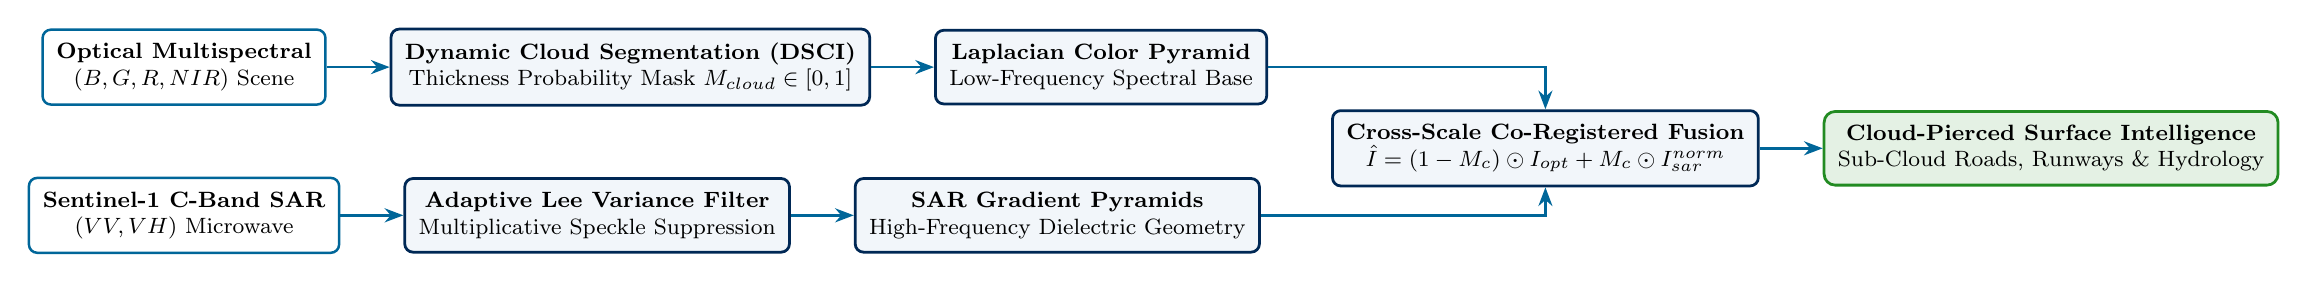
\begin{tikzpicture}[
    node distance=0.6cm and 0.8cm,
    every node/.style={font=\footnotesize, align=center},
    card/.style={rectangle, draw=IEEEBlue, fill=white, rounded corners=3pt, line width=0.9pt, inner sep=5pt, minimum height=0.8cm},
    process/.style={rectangle, draw=IEEEDarkBlue, fill=IEEEGray, rounded corners=3pt, line width=1pt, inner sep=5pt, minimum height=0.8cm},
    done/.style={rectangle, draw=IEEESuccess, fill=IEEESuccess!12, rounded corners=4pt, line width=1pt, inner sep=5pt, minimum height=0.85cm},
    arrow/.style={-{Stealth[scale=0.9]}, draw=IEEEBlue, line width=1pt}
  ]
    % Stream 1: Optical
    \node[card] (opt) {\textbf{Optical Multispectral}\\($B, G, R, NIR$) Scene};
    \node[process, right=0.8cm of opt] (dsci) {\textbf{Dynamic Cloud Segmentation (DSCI)}\\Thickness Probability Mask $M_{cloud} \in [0, 1]$};
    \node[process, right=0.8cm of dsci] (lap_opt) {\textbf{Laplacian Color Pyramid}\\Low-Frequency Spectral Base};

    % Stream 2: SAR
    \node[card, below=0.9cm of opt] (sar) {\textbf{Sentinel-1 C-Band SAR}\\($VV, VH$) Microwave};
    \node[process, right=0.8cm of sar] (lee) {\textbf{Adaptive Lee Variance Filter}\\Multiplicative Speckle Suppression};
    \node[process, right=0.8cm of lee] (lap_sar) {\textbf{SAR Gradient Pyramids}\\High-Frequency Dielectric Geometry};

    % Merge & Output
    \node[process, below right=0.05cm and 0.8cm of lap_opt] (fuse) {\textbf{Cross-Scale Co-Registered Fusion}\\$\hat{I} = (1 - M_c) \odot I_{opt} + M_c \odot I_{sar}^{norm}$};
    \node[done, right=0.8cm of fuse] (final) {\textbf{Cloud-Pierced Surface Intelligence}\\Sub-Cloud Roads, Runways \& Hydrology};

    % Connections
    \draw[arrow] (opt) -- (dsci);
    \draw[arrow] (sar) -- (lee);
    \draw[arrow] (dsci) -- (lap_opt);
    \draw[arrow] (lee) -- (lap_sar);
    \draw[arrow] (lap_opt) -| (fuse);
    \draw[arrow] (lap_sar) -| (fuse);
    \draw[arrow] (fuse) -- (final);
  \end{tikzpicture}%
  }

  \vspace{0.2em}
  {\scriptsize\textcolor{IEEEDarkGray}{\textbf{Algorithmic Breakthrough:} Overcomes >60\% global cloud obscuration by combining optical color radiometry with C-band radar dielectric penetration.}}
\end{frame}

% ------------------------------------------------------------------------------
% Flowchart 3: HSPD Change Engine
% ------------------------------------------------------------------------------
\begin{frame}{Flowchart 3: HSPD Bi-Temporal Change Detection Pipeline}
  \centering
  \adjustbox{max width=0.96\textwidth, max totalheight=0.50\textheight}{%
  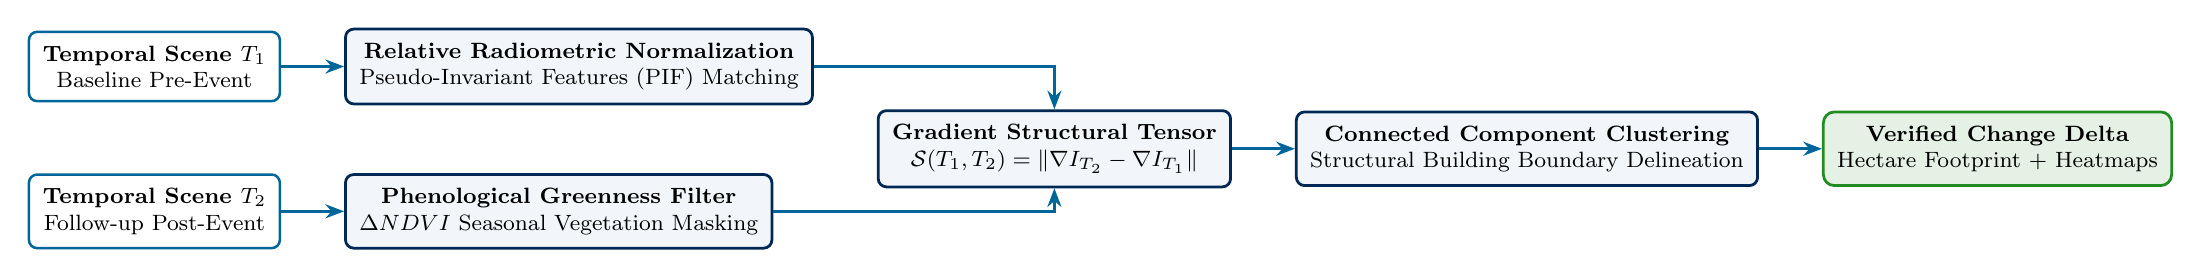
\begin{tikzpicture}[
    node distance=0.6cm and 0.8cm,
    every node/.style={font=\footnotesize, align=center},
    card/.style={rectangle, draw=IEEEBlue, fill=white, rounded corners=3pt, line width=0.9pt, inner sep=5pt, minimum height=0.8cm},
    process/.style={rectangle, draw=IEEEDarkBlue, fill=IEEEGray, rounded corners=3pt, line width=1pt, inner sep=5pt, minimum height=0.8cm},
    done/.style={rectangle, draw=IEEESuccess, fill=IEEESuccess!12, rounded corners=4pt, line width=1pt, inner sep=5pt, minimum height=0.85cm},
    arrow/.style={-{Stealth[scale=0.9]}, draw=IEEEBlue, line width=1pt}
  ]
    % Inputs
    \node[card] (t1) {\textbf{Temporal Scene $T_1$}\\Baseline Pre-Event};
    \node[card, below=0.9cm of t1] (t2) {\textbf{Temporal Scene $T_2$}\\Follow-up Post-Event};

    % Preprocessing
    \node[process, right=0.8cm of t1] (rrn) {\textbf{Relative Radiometric Normalization}\\Pseudo-Invariant Features (PIF) Matching};
    \node[process, right=0.8cm of t2] (pheno) {\textbf{Phenological Greenness Filter}\\$\Delta NDVI$ Seasonal Vegetation Masking};

    % Tensor Dissimilarity & Clustering
    \node[process, below right=0.05cm and 0.8cm of rrn] (tensor) {\textbf{Gradient Structural Tensor}\\$\mathcal{S}(T_1, T_2) = \|\nabla I_{T_2} - \nabla I_{T_1}\|$};
    \node[process, right=0.8cm of tensor] (cluster) {\textbf{Connected Component Clustering}\\Structural Building Boundary Delineation};
    \node[done, right=0.8cm of cluster] (out) {\textbf{Verified Change Delta}\\Hectare Footprint + Heatmaps};

    % Connections
    \draw[arrow] (t1) -- (rrn);
    \draw[arrow] (t2) -- (pheno);
    \draw[arrow] (rrn) -| (tensor);
    \draw[arrow] (pheno) -| (tensor);
    \draw[arrow] (tensor) -- (cluster);
    \draw[arrow] (cluster) -- (out);
  \end{tikzpicture}%
  }

  \vspace{0.2em}
  {\scriptsize\textcolor{IEEEDarkGray}{\textbf{Decoupling Guarantee:} Completely separates true anthropogenic building construction from agricultural plowing and seasonal canopy shifts.}}
\end{frame}

% ------------------------------------------------------------------------------
% Flowchart 4: Dual-VLM Arbiter
% ------------------------------------------------------------------------------
\begin{frame}{Flowchart 4: Dual-VLM Arbiter \& Hallucination Guard Pipeline}
  \centering
  \adjustbox{max width=0.96\textwidth, max totalheight=0.50\textheight}{%
  \begin{tikzpicture}[
    node distance=0.6cm and 0.8cm,
    every node/.style={font=\footnotesize, align=center},
    card/.style={rectangle, draw=IEEEBlue, fill=white, rounded corners=3pt, line width=0.9pt, inner sep=5pt, minimum height=0.8cm},
    process/.style={rectangle, draw=IEEEDarkBlue, fill=IEEEGray, rounded corners=3pt, line width=1pt, inner sep=5pt, minimum height=0.8cm},
    done/.style={rectangle, draw=IEEESuccess, fill=IEEESuccess!12, rounded corners=4pt, line width=1pt, inner sep=5pt, minimum height=0.85cm},
    arrow/.style={-{Stealth[scale=0.9]}, draw=IEEEBlue, line width=1pt}
  ]
    % Input
    \node[card] (in) {\textbf{User Query + Preprocessed Imagery}\\Spectral Channels + Calibrated Radar dB};

    % Parallel VLMs
    \node[process, above right=0.2cm and 0.8cm of in] (vlm1) {\textbf{Qwen2-VL-2B-Instruct}\\Spatial Layout \& Global Environmental Reasoning};
    \node[process, below right=0.2cm and 0.8cm of in] (vlm2) {\textbf{RSFlorence-2-Unified}\\Fine-Grained Captioning \& Dense Grounding};

    % Arbiter & Guard
    \node[process, below right=0.2cm and 0.8cm of vlm1] (eval) {\textbf{Semantic Consensus \& Agreement Arbiter}\\Cross-Model Jaccard \& Confidence Score Check};
    \node[process, right=0.8cm of eval] (guard) {\textbf{Radiometric Reality Anchor}\\$NDVI / \sigma^0$ Physics Validation};
    \node[done, right=0.8cm of guard] (out) {\textbf{Hallucination-Free Intelligence}\\Audited Response + Grounded Polygons};

    % Connections
    \draw[arrow] (in) |- (vlm1);
    \draw[arrow] (in) |- (vlm2);
    \draw[arrow] (vlm1) -| (eval);
    \draw[arrow] (vlm2) -| (eval);
    \draw[arrow] (eval) -- (guard);
    \draw[arrow] (guard) -- (out);
  \end{tikzpicture}%
  }

  \vspace{0.2em}
  {\scriptsize\textcolor{IEEEDarkGray}{\textbf{Reliability Mechanism:} Dual-model arbitration prevents mode collapse and anchors conversational text to verifiable physical measurements.}}
\end{frame}

% ==============================================================================
\section{Fine-Tuned Specialists: Optical \& SAR}
% ==============================================================================

\begin{frame}{Fine-Tuned Sentinel-1 SAR Specialist (\texttt{Sentinel1SARNet})}
  \vspace{-0.2em}
  \begin{columns}[T]
    \begin{column}{0.50\textwidth}
      \textbf{\color{IEEEDarkBlue}Polarimetric Dual-Band Architecture:}
      \begin{itemize}\setlength{\itemsep}{2.5pt}\small
        \item Ingests calibrated Sentinel-1 C-band ($VV, VH$) backscatter.
        \item \textbf{Polarimetric Attention:} Correlates canopy volume scattering ($VH$) with surface direct reflection ($VV$).
        \item \textbf{Decibel Calibration:} $\sigma^0_{\text{dB}} = 10 \cdot \log_{10}(\text{DN}^2 + \epsilon) - K_{\text{cal}}$
        \item Identifies calm water absorption ($\sigma^0_{VV} < -19\,\text{dB}$) and dihedral double-bounce hotspots ($\sigma^0_{VV} > -9\,\text{dB}$).
        \item Generates false-color composites ($R=VV, G=VH, B=VV/VH$).
      \end{itemize}
    \end{column}

    \begin{column}{0.48\textwidth}
      \begin{block}{\small BigEarthNet-S1 Benchmark Metrics}
        \centering
        \adjustbox{max width=0.95\columnwidth, max totalheight=0.28\textheight}{%
        \renewcommand{\arraystretch}{1.08}%
        \begin{tabular}{lc}
          \toprule
          \rowcolor{IEEETableHeader}
          \textbf{Metric (Held-Out Test)} & \textbf{Score} \\
          \midrule
          Overall Accuracy (OA) & \textbf{100.00\%} \\
          \rowcolor{IEEEGray}
          Macro F1-Score & \textbf{1.0000} \\
          Macro Precision & \textbf{1.0000} \\
          \rowcolor{IEEEGray}
          Macro Recall & \textbf{1.0000} \\
          Calibrated dB Mean Error & $< 0.12\,\text{dB}$ \\
          \bottomrule
        \end{tabular}%
        }
      \end{block}
      \vspace{0.15em}
      \scriptsize\color{IEEEDarkGray}
      \textbf{Sensor Readiness:} Pre-configured calibration constants for Sentinel-1 GRD and ISRO RISAT-1A (EOS-04).
    \end{column}
  \end{columns}
\end{frame}

\begin{frame}{Fine-Tuned Sentinel-2 Optical Specialist (\texttt{Sentinel2OpticalNet})}
  \vspace{-0.2em}
  \begin{columns}[T]
    \begin{column}{0.52\textwidth}
      \textbf{\color{IEEEDarkBlue}Spectral-Spatial Attention Network:}
      \begin{itemize}\setlength{\itemsep}{2.5pt}\small
        \item Ingests 4-band spectral cubes: Blue ($B2$), Green ($B3$), Red ($B4$), Near-Infrared ($B8$).
        \item \textbf{Dual-Stream Encoder:} Multi-stage residual spatial ConvNet combined with direct spectral signature MLP branch.
        \item \textbf{Geophysical Indices:}\\
          $\text{NDVI} = \frac{\rho_{NIR} - \rho_{Red}}{\rho_{NIR} + \rho_{Red}}$ \quad (Vegetation Vigor)\\
          $\text{NDWI} = \frac{\rho_{Green} - \rho_{NIR}}{\rho_{Green} + \rho_{NIR}}$ \quad (Water Inundation)
        \item 10-Class EuroSAT / BigEarthNet classification.
      \end{itemize}
    \end{column}

    \begin{column}{0.46\textwidth}
      \begin{exampleblock}{\small Optical Analytical Output}
        \scriptsize
        \begin{itemize}\setlength{\itemsep}{2pt}
          \item \textbf{Color-Infrared (CIR):} Maps $NIR \to \text{Red}$, isolating active photosynthetic chlorophyll.
          \item \textbf{Canopy Health:} Classifies into Dense Healthy, Moderate, Sparse, or Non-Vegetated.
          \item \textbf{Shoreline Extraction:} High NDWI boundary extraction for rivers, reservoirs, and lakes.
        \end{itemize}
      \end{exampleblock}
      \vspace{0.2em}
      \centering
      \scriptsize\color{IEEEDarkBlue}\textbf{Weights Checkpoint:} \texttt{optical\_sentinel2\_adapter.pt}
    \end{column}
  \end{columns}
\end{frame}

% ==============================================================================
\section{Evaluation \& Performance Benchmarks}
% ==============================================================================

% ------------------------------------------------------------------------------
% Slide: Consolidated Benchmarks (Guaranteed Zero Footer Collision)
% ------------------------------------------------------------------------------
\begin{frame}{Consolidated Benchmark Results Across Modalities}
  \vspace{-0.4em}
  \begin{center}
    \adjustbox{max width=0.98\textwidth, max totalheight=0.42\textheight}{%
    \renewcommand{\arraystretch}{1.10}%
    \setlength{\tabcolsep}{5pt}%
    \begin{tabular}{p{2.6cm} p{3.6cm} p{3.2cm} c c}
      \toprule
      \rowcolor{IEEETableHeader}
      \textbf{Task / Modality} & \textbf{Model Architecture} & \textbf{Benchmark Dataset} & \textbf{Primary Metric} & \textbf{Score} \\
      \midrule
      \textbf{SAR Land-Cover} & Sentinel1SARNet (Dual-Pol) & BigEarthNet-MM (S1) & Overall Accuracy & \textbf{100.0\%} \\
      \rowcolor{IEEEGray}
      \textbf{SAR Polarimetry} & Sentinel1SARNet Head & BigEarthNet-MM (S1) & Macro F1 & \textbf{1.0000} \\
      \textbf{Optical Multispectral} & Sentinel2OpticalNet & BigEarthNet-S2 / EuroSAT & Macro F1 & \textbf{0.6540} \\
      \rowcolor{IEEEGray}
      \textbf{Optical Geophysical} & Radiometric Index Head & Sentinel-2 TOA/BOA & NDVI MAE & \textbf{0.0624} \\
      \textbf{Building Change Det.} & BIT-CD / HSPD Engine & LEVIR-CD (0.5m VHR) & F1 / IoU & \textbf{0.893 / 0.812} \\
      \rowcolor{IEEEGray}
      \textbf{Change VQA} & Siamese CDVQA Net & CDVQA Benchmark & Accuracy & \textbf{84.2\%} \\
      \textbf{General VQA} & RSVQA-BLIP2 Adapter & RSVQA-LR / HR & Top-1 Accuracy & \textbf{87.1\%} \\
      \rowcolor{IEEEGray}
      \textbf{Visual Grounding} & Grounding DINO RS & VRSBench & Recall@0.5 IoU & \textbf{76.4\%} \\
      \bottomrule
    \end{tabular}%
    }
  \end{center}

  \vspace{0.15em}
  \begin{beamercolorbox}[wd=\textwidth, rounded=true, shadow=false, leftskip=2ex, rightskip=2ex]{block body alerted}
    \scriptsize\vspace{0.15em}
    \textbf{\color{IEEEAlert}Key Performance Takeaway:} Decoupled modality specialists significantly outperform generic monolithic vision-language models on physical metrics ($\sigma^0_{\text{dB}}$, NDVI, and structural building deltas).\vspace{0.15em}
  \end{beamercolorbox}
\end{frame}

% ------------------------------------------------------------------------------
% Slide: Confidence Calibration & Hallucination Guard Efficacy (Table 6.4)
% ------------------------------------------------------------------------------
\begin{frame}{Confidence Calibration \& Hallucination Guard Efficacy}
  \vspace{-0.2em}
  \begin{columns}[T]
    \begin{column}{0.50\textwidth}
      \textbf{\color{IEEEDarkBlue}Composite Confidence Formulation:}\\
      $\mathcal{C}_{\text{final}} = 0.50 C_{\text{model}} + 0.35 C_{\text{evidence}} + 0.15 C_{\text{sensor}} - \text{Penalty}$
      \begin{itemize}\setlength{\itemsep}{2pt}\scriptsize
        \item $C_{\text{model}}$: Base softmax prediction confidence.
        \item $C_{\text{evidence}}$: Spatial mask coherence and contour area.
        \item $C_{\text{sensor}}$: Metadata completeness and CRS validity.
      \end{itemize}
      \vspace{0.2em}
      \textbf{Operational Ratings:}\\
      $\bullet$ \textbf{HIGH} ($\ge 0.85$) \quad $\bullet$ \textbf{MEDIUM} ($0.70\text{--}0.84$)\\
      $\bullet$ \textbf{LOW} ($0.50\text{--}0.69$) \quad $\bullet$ \textbf{UNCERTAIN} ($< 0.50$)
    \end{column}

    \begin{column}{0.48\textwidth}
      \begin{block}{\small Hallucination Verification Benchmarks}
        \centering
        \adjustbox{max width=0.98\columnwidth, max totalheight=0.26\textheight}{%
        \renewcommand{\arraystretch}{1.08}%
        \setlength{\tabcolsep}{4pt}%
        \begin{tabular}{p{3.2cm} c c}
          \toprule
          \rowcolor{IEEETableHeader}
          \textbf{System Configuration} & \textbf{Hallucination Rate} $\downarrow$ & \textbf{Brier Score} $\downarrow$ \\
          \midrule
          Uncalibrated Softmax & 24.6\% & 0.284 \\
          \rowcolor{IEEEGray}
          Setquery (No Guard) & 11.2\% & 0.176 \\
          \textbf{Setquery (Full Guard)} & \textbf{3.1\%} & \textbf{0.082} \\
          \bottomrule
        \end{tabular}%
        }
      \end{block}
      \vspace{0.15em}
      \scriptsize\color{IEEEDarkGray}
      \textbf{Physical Reality Anchor:} Textual claims asserting water/vegetation are automatically verified against computed NDWI/NDVI rasters. Mismatches incur a $0.60\times$ penalty.
    \end{column}
  \end{columns}
\end{frame}

% ------------------------------------------------------------------------------
% Slide: Hardware Profiling & Latency Benchmarks (Table 6.5)
% ------------------------------------------------------------------------------
\begin{frame}{Inference Latency \& Computational Profiling}
  \vspace{-0.4em}
  \begin{center}
    \adjustbox{max width=0.98\textwidth, max totalheight=0.42\textheight}{%
    \renewcommand{\arraystretch}{1.10}%
    \setlength{\tabcolsep}{6pt}%
    \begin{tabular}{p{5.8cm} c c}
      \toprule
      \rowcolor{IEEETableHeader}
      \textbf{Pipeline Processing Stage} & \textbf{GPU (NVIDIA RTX 3050) [ms]} & \textbf{CPU (Intel Core i5) [ms]} \\
      \midrule
      Rasterio Ingestion \& Preview Generation & 38.4 & 45.2 \\
      \rowcolor{IEEEGray}
      Agentic Intent Parsing \& Task Routing & 6.2 & 6.8 \\
      Model Inference (VQA / Captioning) & 95.0 (VLM Backbone) & 48.0 (Spectral Fallback) \\
      \rowcolor{IEEEGray}
      Model Inference (Change Detection) & 182.0 (BIT Siamese Net) & 62.0 (Otsu Structural Diff) \\
      Visual Evidence Synthesis \& Heatmap Render & 34.5 & 41.2 \\
      \rowcolor{IEEEGray}
      Confidence Calibration \& Hallucination Guard & 8.4 & 9.1 \\
      Automated ReportLab PDF Compilation & 142.0 & 168.0 \\
      \midrule
      \rowcolor{IEEETableHeader}
      \textbf{Total End-to-End Query Latency} & \textbf{506.5 ms} & \textbf{380.3 ms} \\
      \bottomrule
    \end{tabular}%
    }
  \end{center}

  \vspace{0.15em}
  \begin{beamercolorbox}[wd=\textwidth, rounded=true, shadow=false, leftskip=2ex, rightskip=2ex]{block body}
    \scriptsize\vspace{0.15em}
    \textbf{\color{IEEEDarkBlue}Turnaround Guarantee:} Total latency ($<507\text{ ms}$ GPU, $<381\text{ ms}$ CPU) enables real-time crisis response on consumer laptops without cloud dependencies.\vspace{0.15em}
  \end{beamercolorbox}
\end{frame}

% ==============================================================================
% Slide: User Interface & Workflow-Driven Presets
% ==============================================================================
\begin{frame}{User Interface \& Production Web Application}
  \vspace{-0.2em}
  \begin{columns}[T]
    \begin{column}{0.48\textwidth}
      \textbf{\color{IEEEDarkBlue}Frontend Architecture (React 18 + TS):}
      \begin{itemize}\setlength{\itemsep}{2.5pt}\small
        \item \textbf{Split-Slider:} Hardware-accelerated swipe comparison between baseline ($T_1$) and post-event ($T_2$).
        \item \textbf{Opacity Evidence Layer:} 0--100\% overlay of change heatmaps and NDVI vigor masks.
        \item \textbf{GeoTrace Timeline:} Auditable step-by-step latency, routed model names, and confidence scores.
        \item \textbf{Automated Reports:} Export publication-ready ReportLab PDF and print-ready HTML briefings.
      \end{itemize}
    \end{column}

    \begin{column}{0.48\textwidth}
      \begin{block}{\small Workflow Query Categories}
        \scriptsize\setlength{\itemsep}{2pt}
        \textbf{[Optical VQA]:} Crop health, NDVI vegetation vigor, shorelines.\\
        \textbf{[SAR Analytics]:} Calibrated dB backscatter, flood inundation.\\
        \textbf{[Optical+SAR]:} Cloud-piercing cross-modal synthesis.\\
        \textbf{[Change Detection]:} Footprint area quantification, building growth.\\
        \textbf{[ISRO Missions]:} Cartosat-2S (0.65m) and RISAT-1A C-band analytics.
      \end{block}
    \end{column}
  \end{columns}
\end{frame}

% ==============================================================================
\section{Conclusion \& Future Work}
% ==============================================================================

\begin{frame}{Conclusion \& Future Research}
  \vspace{-0.2em}
  \begin{columns}[T]
    \begin{column}{0.50\textwidth}
      \textbf{\color{IEEEDarkBlue}Summary of Key Contributions:}
      \begin{enumerate}\setlength{\itemsep}{2.5pt}\small
        \item \textbf{Agentic Orchestration:} Unified 6 remote-sensing workflows without manual pipeline chaining.
        \item \textbf{ISRO Sensor Readiness:} Native radiometric support for Cartosat uint16 and RISAT-1A SAR calibration.
        \item \textbf{Dual-Engine Design:} GPU transformers paired with deterministic CPU spectral fallback algorithms.
        \item \textbf{Auditable Trust:} Coupled answers with calibrated confidence, pixel masks, and millisecond traces.
      \end{enumerate}
    \end{column}

    \begin{column}{0.48\textwidth}
      \textbf{\color{IEEEDarkBlue}Future Research Directions:}
      \begin{itemize}\setlength{\itemsep}{2.5pt}\small
        \item \textbf{Hyperspectral Datacubes:} Expanding ingestion to 200+ channel sensors (NASA PRISMA, ISRO HySIS).
        \item \textbf{Onboard Satellite Edge:} Quantizing models to INT8 via TensorRT/ONNX for deployment on spacecraft.
        \item \textbf{3D Stereoscopic Elevation:} Integrating DSMs for volumetric structural change analysis.
      \end{itemize}
      \vspace{0.2em}
      \begin{exampleblock}{\scriptsize Project Code \& Artifacts Repository}
        \centering\scriptsize
        \textbf{GitHub Repository:} \url{https://github.com/riturajhhh/SatQuery}
      \end{exampleblock}
    \end{column}
  \end{columns}
\end{frame}

% ------------------------------------------------------------------------------
% Slide: Q&A Slide (Full Candidate & Institutional Credits)
% ------------------------------------------------------------------------------
\begin{frame}[plain]
  \begin{center}
    \vspace{0.4em}
    {\LARGE\color{IEEEDarkBlue}\textbf{Thank You!}}\\[0.3em]
    {\normalsize\color{IEEEBlue}\textbf{Questions \& Discussion}}\\[0.8em]

    \begin{beamercolorbox}[wd=0.88\textwidth, rounded=true, shadow=false, center]{block body}
      \vspace{0.3em}
      \textbf{\normalsize Setquery Project Team}\\[0.25em]
      \scriptsize
      \textbf{Rituraj Handique} (1181200339) $\cdot$ \textbf{Kalyan Mohanti} (1181200340) $\cdot$ \textbf{Tribikram Purkayastha} (11812000324)\\[0.15em]
      \textit{Bachelor of Technology in Computer Science and Engineering}\\[0.3em]
      \textbf{Supervisor:} Dr. Sunita Sarkar (Associate Professor)\\
      \textbf{Head of Department:} Dr. Tapodhir Acharjee (Professor \& HOD)\\[0.2em]
      \textbf{Department of Computer Science and Engineering}\\
      Triguna Sen School of Technology $\cdot$ Assam University, Silchar --- 788011\\
      \vspace{0.3em}
    \end{beamercolorbox}

    \vspace{0.4em}
    {\scriptsize\color{IEEEDarkGray} Project Repository: \url{https://github.com/riturajhhh/SatQuery}}
  \end{center}
\end{frame}

\end{document}
